\chapter{Project Management}


\section{Planning}

\begin{tabular}{ l l l }
    \hline
    \bold{\textnumero} & \bold{Milestone}                       & \bold{Date of Achieval} \\ \hline
    MS\_1              & Cultivation of Bacteria                & 09.11.2023              \\
    MS\_2              & Extraction of LanM                     & 07.12.2023              \\
    MS\_3              & Detection of LanM                      & n/d                     \\
    MS\_4              & Binding of LanM to Rare Earth Elements & n/d                     \\
    MS\_5              & Separation of Rare Earths from LanM    & n/d                     \\
    \hline
\end{tabular}


\section{Evaluation\authorA{}}
When we started to conduct some research for the project in the summer break, we also began simultaneously to plan the work with agile project management methods.
As it turned out, doing the project management this way was really helpful.
During our work, we encountered a lot of obstacles which we had not thought of before, which resulted in a slower progress than we had previously expected.
Using an agile project board made it very easy for us to keep track of all of our work.
Even though on some days we had to add more tasks to the \emph{Todo} or \emph{In Progress} than to the \emph{Finished} section.

\begin{figure}[H]
    \centering
    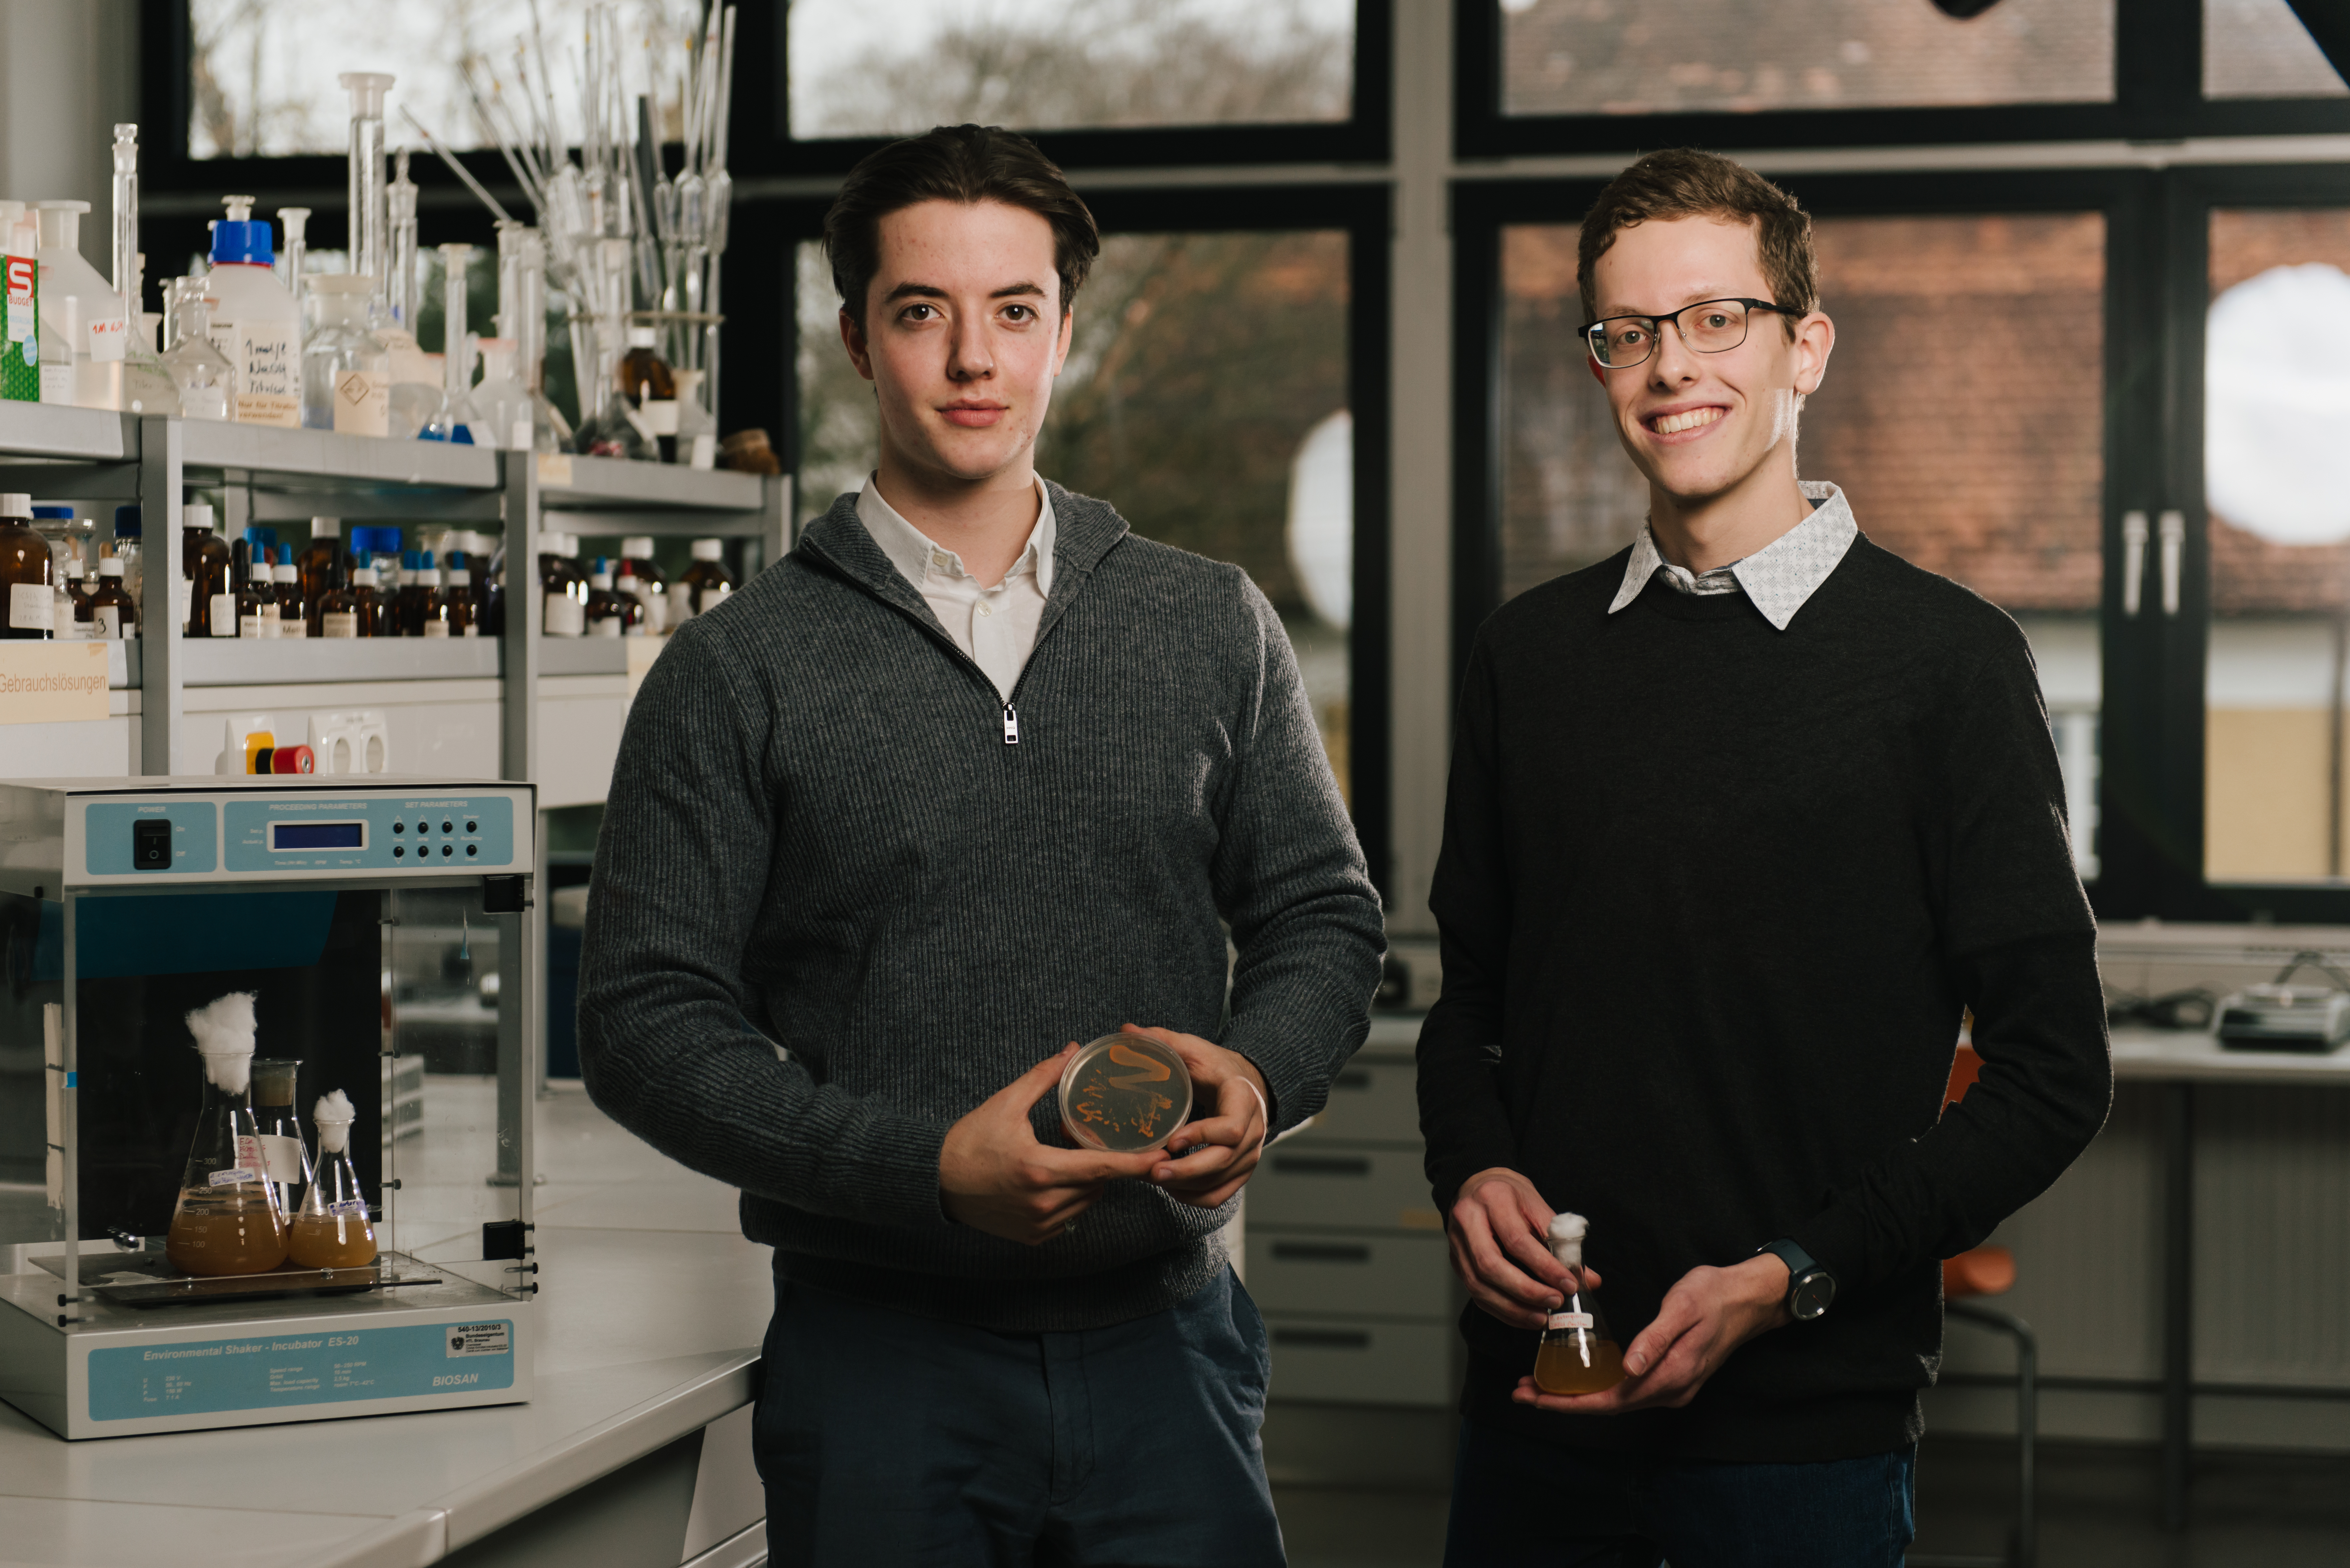
\includegraphics[width=0.75\textwidth]{./media/images/teamfoto}
    \caption{The project team}
    \label{fig:teamphoto}
\end{figure}

\newpage


\section{Timesheet}

\subsection{Tobias Daxecker}


\begin{tabularx}{\textwidth}{l p{1cm} l p{1cm} X}

    Braunau/Inn, \todayshort & & Tobias Daxecker & & \hrulefill                       \\
    \emph{Ort, Datum}        & &                 & & \emph{Unterschrift} \vspace{2cm} \\

\end{tabularx}

\subsection{Mathias Standhartinger}

\begin{tabularx}{\textwidth}{l p{1cm} l p{1cm} X}

    Braunau/Inn, \todayshort & & Mathias Standhartinger & & \hrulefill                       \\
    \emph{Ort, Datum}        & &                        & & \emph{Unterschrift} \vspace{2cm} \\

\end{tabularx}

